\chapter{Analytical techniques}
\label{ch:analyticaltechniques}

Isotope geochemistry is based on the accurate and precise
determination of elemental and isotopic compositions of rocks and
minerals.  Although some of the earliest geochronological methods
(notably the $^{14}$C method, see Section \ref{sec:14C}) were based on
the detection of radioactivity by means of Geiger-M\"{u}ller counters
and liquid scintillation detectors, nearly all modern isotope
geochemistry is done by mass spectrometry.

\section{Mass spectrometry}
\label{sec:mass-specs}

A mass spectrometer is a device that separates electrically charged
atoms or molecules based on their mass, enabling precise measurement
of the isotopic composition. A mass spectrometer consists of the
following parts:

\begin{enumerate}
\item ion source: this can be either a filament (similar to that found
  in an incandescent light bulb), a plasma torch, a primary ion beam,
  or a spray chamber, among other possibilities.
\item mass analyser: this can be an electromagnet (possibly combined
  with an electrostatic field), or a rapidly fluctuating electric
  field.
\item ion detector: this is, essentially, a volt meter.
\end{enumerate}

In the remainder of this section, we will assume the source to be a
filament and the mass analyser to be an electromagnet. \\

After pumping the mass spectrometer down to (ultra-)high vacuum
conditions (10$^{-6}$ to 10$^{-9}$ mbar), the sample enters the ion
source as a gas, where it is bombarded with electrons.  The resulting
ions (with charge $e$) are accelerated in an electric field (with
potential difference $V$) and collimated to a narrow beam. This beam
is sent through a magnetic field (with strength $H$) which deflects it
into a circular trajectory with a radius proportional to the ion mass
($m$).  This results in a physical separation of the incoming ion beam
into various outgoing beams. The beams of interest are steered into
the ion detector which, in its simplest design (the so-called `Faraday
Cup') consists of a long and narrow cup. The ion beam is neutralised
in the cup by electrons flowing from ground through a resistor. The
potential difference across this resistor is measured and registered
on a computer for further processing.\\

The electric field transfers a certain amount of kinetic energy to the
ions:

\begin{equation}
E = e V = \frac{m v^2}{2}
\label{eq:E}
\end{equation}

With $e$ is the electrical charge (in multiples of 1.60219 $\times
10^{-19}$C, which is the elementary charge of an electron.  Because
each type of ion has a different mass ($m$, in multiples of 1.660538
$\times 10^{-27}$kg, the atomic mass unit), their terminal velocity
($v$) differs as well:

\begin{equation}
v = \sqrt{\frac{2 e V}{m}}
\label{eq:v}
\end{equation}

The mass analyser deflects the ions according to the following equation:

\begin{equation}
H e v = \frac{m v^2}{r}
\label{eq:Hev}
\end{equation}

Substituting Equation \ref{eq:v} into \ref{eq:Hev} yields:

\begin{equation}
H \sqrt{\frac{2 e V}{m}} = \frac{2 V}{r}
\label{eq:H2eVm}
\end{equation}

from which it follows that:

\begin{equation}
\begin{array}{rl}
~ & r = \frac{1}{H}\sqrt{\frac{2 m V}{e}} \\
\mbox{and}~ & H = \frac{1}{r}\sqrt{\frac{2 m V}{e}}\\
\end{array}
\label{eq:rH}
\end{equation}

Equation \ref{eq:rH} allows us to calculate the radius of the ion
trajectory for any given mass-to-charge ratio $m/e$. Note that light
isotopes are more strongly deflected than equally charged heavy ones.
Equation \ref{eq:rH} can also be used to calculate the magnetic field
strength required to deflect an ion beam with a given $m/e$ ratio into
the collector.  This is more practical because most mass spectrometers
have a fixed radius so that the different ions must be collected by
varying $H$. Some modern mass spectrometers are equipped with multiple
ion collectors the enabling simultaneous analysis of several ionic
masses.

\begin{figure}[!ht]
  \centering
  \ifpdf
  \def\svgwidth{\textwidth}
  \input{mass-spec.pdf_tex}
  \else
  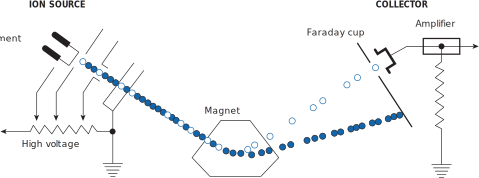
\includegraphics[width=10cm]{../figures/mass-spec.png}
  \fi
  \caption{Schematic diagram of a sector-field noble gas or TIMS mass
    spectrometer \citep[modified from][]{allegre2008}.}
  \label{fig:mass-spec}
\end{figure}

Several types of mass spectrometers are used for geoscience
applications:

\begin{enumerate}
\item{\emph{Thermal Ionisation Mass Spectrometry (TIMS)}.}\\ The
  sample is dissolved and subjected to careful chemical separation
  procedures (liquid chromatography) in order to separate the parent
  and daughter elements to a high level of purity. The resulting
  solutions are spiked and deposited on a tungsten or tantalum
  filament, which is brought to a glow by an electric current and thus
  produces ions. These are separated by a large electromagnet and
  analysed in one or more Faraday cups. TIMS is very time consuming
  but produces extremely precise results (\permil-level precision on
  the ages).
 
\item{\emph{Inductively Coupled Plasma Mass Spectrometry
    (ICP-MS)}.}\\ The sample is vapourised in one of two ways: either
  by introducing a liquid into a spray chamber, or by firing an
  ultraviolet laser at a solid sample and transporting the resulting
  aerosol into the ion source with a carrier gas (typically
  helium). The ion source itself consists of an argon flow which is
  heated to a temperature of approximately 10,000K by sending a
  radiofrequency current through a coil. This breaks up all the
  molecular bonds and produces a plasma (i.e. a `soup' of ions and
  electrons) which enters the high vacuum chamber through a tiny
  opening.  The mass analyser can either be a sector magnet or a
  quadrupole (which consists of four metal rods generating a rapidly
  fluctuating electrical field). ICP-MS offers a higher throughput
  than TIMS, especially in laser ablation mode, where hundreds of ages
  can be measured per day. However, this increased throughput comes at
  the expense of precision, which is on the percent level (better in
  solution mode).

\item{\emph{Secondary ion mass spectrometry (SIMS)}}\\ Prior to the
  development of laser ablation (LA-) ICP-MS, the only other method to
  produce spot measurements in solid samples was by firing a beam of
  negative (e.g. oxygen) or positive (e.g. caesium) ions at the target
  under high vacuum.  This releases (`sputters') positive (or
  negative, in the case of a Cs beam) \emph{secondary} ions from the
  sample surface, which are accelerated by an electrostatic field and
  sent to a sector field mass spectrometer. Although SIMS has been
  replaced by LA-ICP-MS in some applications, it remains an important
  instrument in the geochronological toolbox because (a) it offers
  higher spatial resolution than laser ablation (5-10$\mu m$
  vs. 25-50$\mu m$) and (b) can measure light ions (e.g, hydrogen)
  more reliably than LA-ICP-MS.

\item{\emph{Noble gas mass spectrometry}}\\ The noble gases (He, Ne,
  Ar, Kr, Xe) require a different class of mass spectrometer than the
  rest of the periodic table because, as their name suggests: 1) they
  are gases 2) that do not ionise easily. Noble gasses are liberated
  from solid state materials by heating or laser ablation under
  ultra-high vacuum conditions. To remove any unwanted gas species
  (such as CO, CO\textsubscript{2}, hydrocarbons, etc.) that may
  interfere with the noble gas measurements, the released gas is
  exposed to reactive metals, liquid N\textsubscript{2} `cold traps'
  and other `gettering' devices in a `noble gas extraction line' for a
  duration of 5--30 minutes. The extraction line removes all the
  reactive gas species until only the inert noble gases remain. It is
  only after this lengthy delay that the purified noble gases are
  ionised by electron bombardment, and analysed on the actual mass
  spectrometer.
  
\item{\emph{Accelerator Mass Spectrometer (AMS)}}\\ The AMS combines
  two mass spectrometers with a (`tandem' type) particle accelerator.
  Ions are produced by a SIMS source and steered through a first mass
  analyser, which selects all ions of a desired mass (e.g., mass 14:
  $^{14}$C$^-$, ${}^{12}$CH$_2^-$, $\cdots$). The resulting beam is
  accelerated in the first part of the tandem accelerator by a
  potential difference of several million eV, and sent through a thin
  chamber filled with a `stripper' gas. Collisions of stripper gas
  atoms with the incoming ions destroys any molecular bonds and forms
  3+ ions in the process. The beam now consists of purely atomic ions,
  which are accelerated in the second part of the accelerator and
  steered into a second mass analyser. The AMS has revolutionised the
  $^{14}$C method by enabling the analysis of extremely small
  (mg-sized) samples (see Section \ref{sec:14C}), and has enabled a
  whole new field of geochronology based on the analysis of
  terrestrial cosmogenic radionuclides\ifuclnotes (Chapter
  \ref{sec:cosmo})\fi. The main limitation of AMS is its high
  cost. Currently only two AMS facilities are operating in the UK (in
  Oxford and Glasgow).
\end{enumerate}

\begin{figure}[!ht]
  \centering
  \ifpdf
  \def\svgwidth{\textwidth}
  \input{AMS.pdf_tex}
  \else
  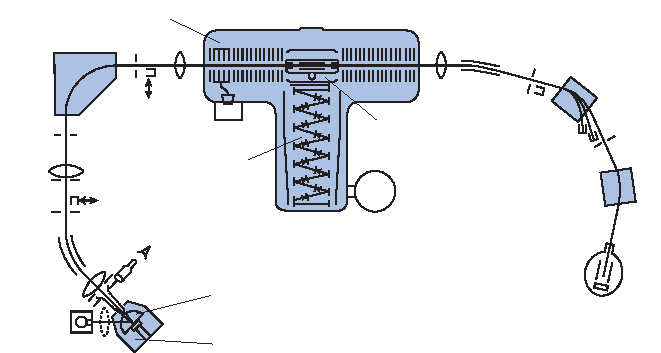
\includegraphics[width=10cm]{../figures/AMS.png}
  \fi
  \caption{Schematic diagram of an Accelerator Mass Spectrometer (AMS)
    \citep[modified from][]{allegre2008}.}
  \label{fig:AMS}
\end{figure}

\section{Isotope dilution}
\label{sec:isotope-dilution}

Besides determining isotopic compositions, the mass spectrometer can
also be used to measure elemental concentrations, using a method
called \emph{isotope dilution}. This is done by mixing the sample
solution (whose isotopic composition has already been determined) with
a known quantity of a solution with a different (but known) isotopic
composition and known elemental concentration. The latter solution is
called the \emph{spike}.  The isotopic composition of the mixture is
analysed by mass spectrometry.  The measured isotopic ratio $R_m$ for
an element with two isotopes ($^aX$ and $^{b}X$) is given by:

\begin{equation}
R_m = \frac{N {}^aX_N + S {}^aX_S}{N {}^bX_N + S {}^bX_S}
\label{eq:Rm}
\end{equation}

with

\begin{equation*}
\begin{array}{rl}
N = & \mbox{the number of atoms of X in the sample}\\
S = & \mbox{the number of atoms of X in the spike}\\
^aX_N, {}^bX_N = & \mbox{the atomic abundance of isotope~} a \mbox{~(or b) in the~}\\
{}^aX_S, {}^bX_S ~~~ & \mbox{sample (or spike)} (^aX_N + {}^bX_N = {}^aX_S + {}^bX_S = 1)
\end{array}
\end{equation*}

$N$ is the only unknown in Equation \ref{eq:Rm}, which can therefore be
rewritten as:

\begin{equation}
N = S \frac{^aX_S - R_m {}^bX_S}{R_m {}^bX_N - {}^aX_N}
\label{eq:N}
\end{equation}

$N$ can also be expressed as a function of the isotopic ratios in the
sample $R_N (={}^aX_N/{}^bX_N)$ and in the spike $R_S
(={}^aX_S/{}^bX_S)$. The atomic abundance of $^aX$ and $^bX$ in the
sample are given by:

\begin{equation}
^aX_N = \frac{R_N}{R_N + 1} \mbox{~and~} {}^bX_N = \frac{1}{R_N + 1}
\label{eq:aXNbXN}
\end{equation}

and in the spike:

\begin{equation}
^aX_S = \frac{R_S}{R_S + 1} \mbox{~and~} {}^bX_S = \frac{1}{R_S + 1}
\label{eq:aXSbXS}
\end{equation}

Substituting Equations \ref{eq:aXSbXS} and \ref{eq:aXNbXN} into
\ref{eq:N} yields:

\begin{equation}
N = S \frac{(R_N+1)(R_S-R_m)}{(R_S+1)(R_m-R_N)}
\label{eq:N2}
\end{equation}

Equations \ref{eq:N} and \ref{eq:N2} give the atomic concentration of
$X$ (in atoms/g).  Dividing $N$ by Avogadro's number $N_A$ and
multiplying with the atomic weights (g/mol) yields the corresponding
weight percentages. Isotope dilution is a very powerful method
because:

\begin{enumerate}
\item It does not require quantative separation of the elements of
  interest.
\item Chemical purification removes unwanted interferences from other
  species.
\item The method is very sensitive, so extremely low concentrations
  can be measured (ppb or less).
\end{enumerate}

\section{Sample-standard bracketing}
\label{sec:bracketing}

Isotope dilution is the `gold standard' for isotope geochemistry,
recommended when the most accurate and precise results are
desired. Unfortunately, isotope dilution is also very time consuming
and cannot be readily applied to micro-analytical techniques such as
LA-ICP-MS and SIMS. In those cases, and alternative method is used,
which is less precise (\%- rather than \permil- level precision) but
quicker.  The idea is to normalise the signal ratios recorded by the
mass spectrometer to a standard of known age.  As before, let P be a
radioactive parent which decays to a radiogenic daughter D. Suppose
that we can measure both nuclides on the same mass spectrometer,
yielding two electronic signal intensities $S_P$ and $S_D$. These
signals may be recorded in units of V, A, or Hz. We cannot directly
use the signal ratios as a proxy for the isotopic ratio:

$$\frac{D}{P} \neq \frac{S_D}{S_P}$$

because the parent and daughter are two different elements with
different chemical properties and ionisation efficiencies. We can,
however, assume that the isotopic ratio is proportional to the signal
ratio:

\begin{equation}
\frac{D}{P} = C \frac{S_D}{S_P}
\label{eq:eqC}
\end{equation}

Thus, if we double $D$ (and thus $D/P$), we would also expect to
double $S_D$ (and thus $S_D/S_P$). To determine the constant of
proportionality $C$, we analyse a standard of known age ($t_s$) and,
hence ($D/P$)-ratio (due to Equation \ref{eq:D}):

\begin{equation}
C = \left(e^{\lambda_Pt_s} - 1\right) \frac{S^s_P}{S^s_D}
\label{eq:const}
\end{equation}

where $\lambda_P$ is the decay constant of the parent and
$S^s_P/S^s_D$ is the (inverse) signal ratio of the standard.
